\documentclass[twocolumn]{article}

%% Language and font encodings
\usepackage[english]{babel}
\usepackage[utf8]{inputenc}
\usepackage{csquotes}
\bibliographystyle{unsrt}
\usepackage{booktabs}

\usepackage{tabu}
\usepackage[T1]{fontenc}

%% Sets page size and margins
\usepackage[a4paper,top=2cm,bottom=2cm,left=3cm,right=3cm,marginparwidth=1.75cm]{geometry}

%% Useful packages
\usepackage{amsmath}
\usepackage{graphicx}
%\usepackage{apacite}
\usepackage[colorinlistoftodos]{todonotes}
\usepackage[colorlinks=true, allcolors=blue]{hyperref}

\title {Simple Model to Track the Rate of Spread of CoronaVirus (COVID-2019) Cases}
\author{Shadrack Jabes, B.}
\date{\it{\today}}

\begin{document}
\maketitle
\section{Introduction}
Here is a simple example of how one can track the rate of spread and to realize how important is this to care for the quarantines and isolations. 
\section{Dataset} 
On the 12th March 2020, there were globally 59212 active cases and 75364 closed cases whilst 13th March 2020, there were 67521 active cases and 77962 closed cases reported. The percentage of increase from 12th March to 13th March can be easily calculated. i.e, 14.1\% and 3.4\% on active and closed cased respectively. In order to find the day with which at this rate of activity to reach the closed case or vice versa, the concept of the differential equation helps here to see how are the viruses along with humans as a carrier controlled without any external support (see figure \ref{fig:dataset}).
                \begin{figure}
                \centering
                \includegraphics[clip=true,trim=0cm 0cm 0cm
                0cm,width=8cm]{ps.predict.active.ps}\\
                        \vspace{-1.43cm}
                \includegraphics[clip=true,trim=0cm 0cm 0cm
                0cm,width=8cm]{ps.predict.closed.ps}
                        \caption{The number of active (top) and closed (bottom) cases as a function of days. The dotted values shown in green represents the actual data and the violet line is the prediction. The functional form used is $f(x) = a_0 + a_1(x^2)$. The coefficients of the functional form for (top) are $a_0$ = 0.953233*$s_{active}$ and $a_1$ = 0.04676*$s_{active}$ and (bottom) are $a_0$ = 0.9885*$s_{closed}$ and $a_1$ = 0.0115*$s_{closed}$. Here, $s_{active}$ and $s_{closed}$ are the number of active and closed cases on day 1 respectively. According to this model, the number of active cases in a month's time will be nearly 3 million and the closed clases will be 0.93 million.}
                \label{fig:dataset}
                \end{figure}
Using this model I used to predict the number of active and recovered cases in each states in India.
\section{Web scrapping}
I scrapped the data from the goverment website in india about the CORONA virus https://www.mygov.in/covid-19. From this website I extract the necessary information on the number of active and closed COVID cases in each of the states in India.
\subsection{Daily updates: cronjob}
I use {\it crontab} to extract the above mentioned information twice every day. This information is stored in ASCII format in my machine. So my computer takes care of extracting the data from the website, analysing the data, running the octave code and computing the parameters for the model described below and then plotting the graph and updating. The following is how it looks (see figure \ref{fig:givendata})\\
		\begin{figure}[htbp]
                \centering
                \includegraphics[clip=true,trim=0cm 0cm 0cm 0cm,width=6cm]{data_covid19.ps}
		\caption{number of active and recovered cases in each states in India on 2020-05-20 according to the goverment website  https://www.mygov.in/covid-19}
                \label{fig:givendata}
                \end{figure}
\section{Nonlinear regression: Machine learning}
{\it Model:} For a given day, we now know the number of active cases. For example: In tamil nadu on 11th May 2020 the number of active cases is 4667. I compare this information with the data obtained yesterday and compute rate of active cases. I assume that the increase in the number of cases, $N$ can be modeled as $N^2$. I use machine learning to compute the paramters with lowest cost function that predicts the number of active cases. Using this model and the parameters I predict what the number of active cases on the scale of a month.
The following is how it looks (see figure \ref{fig:prediction})\\
		\begin{figure}[htbp]
                \centering
                \includegraphics[clip=true,trim=0cm 0cm 0cm 0cm,width=8cm]{predict_covid19.ps}
		\caption{prediction of the number of active and recovered cases on the scale of a month in India}
                \label{fig:prediction}
                \end{figure}
\end{document}
